\section{Zielsetzung}
Ziel des Versuches ist es die Brennweite $f$ von verschiedenen Linsen mit zwei Methoden zu bestimmen. Dazu wird zunächst das Abbildungsgesetz und die Linsengleichung verifiziert. Zusätzlich wird die chromatische Abberation untersucht.

\section{Theoretische Grundlage}
Die in der geometrischen Optik verwendeten Linsen werden in zwei Gruppen eingeteilt: \\
\textbf{1. Sammellinsen}, siehe Abbildung \eqref{fig:Bildkonstruktion} oberes Bild (dünne Linse) und unteres Bild (dicke Linse). Durch die konvexe Wölbung der Sammellinse wird paralleles Licht im so genannten Brennpunkt gebündelt. "Die Brennweite $f$ und die Bildweite $b$ sind bei Sammellinsen positiv und es entseht ein reelles Bild" (\cite{sample}, TU Dortmund, Versuch 408, S.1, 14.05.16). \\
\textbf{2. Zerstreuungslinsen}, siehe Abbildung \eqref{fig:Bildkonstruktion} mittleres Bild (dünne Linse). Sie unterscheidet sich von der Sammellinse durch ihre konkave Wölbung, wodurch das Licht gestreut wird. "Bei einer Zerstreuungslinse sind [die] Brennweite $f$ und [die] Bildweite $b$ negativ und es ensteht ein virtuelles Bild" (\cite{sample}, TU Dortmund, Versuch 408, S.1, 14.05.16). \\
\textbf{Gemeinsamkeiten der beiden Linsenarten:}
\begin{itemize}
	\item Linsen bestehen im allgemeinen aus einem Material welches einen höheren Brechungsindex als Luft aufweist.
	\item Sammel- und Zerstreuungslinsen können in dünne und dicke Linsen eingeteilt werden:
	\begin{itemize}
		\item Für dünne Linsen gilt, dass die Brechung auf die Mittelebene reduziert wird.
		\item Anders als bei den dünnen Linsen muss für dicke Linsen eine zweite Hauptebene eingeführt werden, an welcher der Lichtstrahl gebrochen wird.
	\end{itemize}
	\item Um das Bild zu konstruieren welches nach der Brechung entsteht werden drei Strahlen verwendet (Folgende Auflistung ist entommen aus \cite{sample}, TU Dortmund, Versuch 408, S.1, 14.05.16):
	\begin{itemize}
		\item \textbf{Der Parallelstrahl [$P$]} verläuft vom Gegenstand parallel zur optischen Achse und wird an der Mittelebene bzw. Hauptebene der Linse gebrochen und wird zum Brennpunktstrahl.
		\item \textbf{Der Mittelpunktsstrahl [$M$]} geht durch die Mitte der Linse und ändert seine Richtung nicht.
		\item \textbf{Der Brennpunktsstrahl [$B$]} geht durch den Brennpunkt der Linse, bevor er an der Mittelebene bzw. Hauptebene gebrochen wird und zum Parallelstrahl wird.
	\end{itemize}
\end{itemize}

\begin{figure}[H]
	\centering
	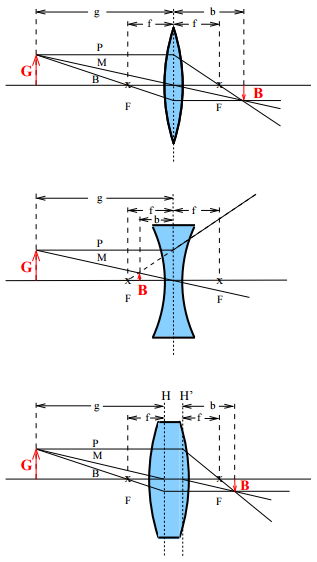
\includegraphics[height=13cm]{picture/Bild1}
	\caption{Bildkonstuktion für drei ausgewählte Linsen. \cite[1]{sample}}
	\label{fig:Bildkonstruktion}
\end{figure}

Das Abbildungsgesetz folgt aus der Abbildung \eqref{fig:Bildkonstruktion} und den Strahlensätzen
\begin{equation}
	V = \frac{B}{G} = \frac{b}{g} \ .
	\label{eqn:V}
\end{equation}
Folgende Bedeutung steckt hinter den Parametern:
\begin{itemize}
	\item $V$: Abbildungsmaßstab
	\item $B$: Bildgröße
	\item $G$: Gegenstandsgröße
	\item $b$: Bildweite
	\item $g$: Gegenstandsweite
\end{itemize}
Das Verhältnis zwischen $B$ und $G$ ist gleich dem Verhältnis von $b$ und $g$, wobei dieses Verhältnis $V$ darstellt. \\
Die Linsengleichung für dünne Linsen kann aus der Bildkonstruktion und dem Abbildungsgesetz hergeleitet werden
\begin{equation}
	\frac{1}{f} = \frac{1}{b} + \frac{1}{g} \ .
	\label{eqn:D}
\end{equation}
Für dicke Linsen kann die Brechung nicht mehr auf eine Mittelebene reduziert werden. Wie die Abbildung \eqref{fig:Bildkonstruktion} unten zeigt, muss die Mittelebene gegen zwei Hauptebenen $H$ und $H'$ ausgetauscht werden. \\
Bei der Gleichung \eqref{eqn:D} handelt es sich um eine Näherung, welche nur gilt solange es um achsennahe Lichstrahlen geht. Durch achsenferne Strahlen können Abbildungsfehler auftreten, wodurch das Bild unscharf abgebildet wird. Das Bild wird wieder scharf, indem mit einer Irisblende die achsenfernen Strahlen ausgeblendet werden. \\
Da der Brechungsindex von der Wellenlänge des eintreffenden Lichtes abhängt, wird blaues Licht stärker gebrochen als rotes. Dieses Phänomen wird chromatische Abberration genannt.

\subsection{Verfahren nach Bessel}
Die Brennweite einer Linse wird nach dem Bessel-Verfahren bestimmt, indem der Abstand zwischen Gegenstand und Bild konstant gehalten wird und zwei Linsenpositionen gesucht werden, bei denen das Bild scharf abgebildet wird
(vgl. \cite{sample}, TU Dortmund, Versuch 408, S.3, 14.05.16).

\begin{figure}[H]
	\centering
	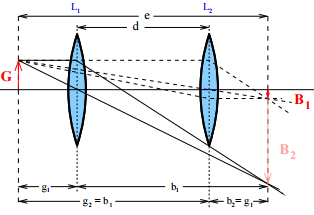
\includegraphics[height=6cm]{picture/Bessel}
	\caption{Schematische Drastellung für das Verfahren von Bessel. \cite[4]{sample}}
	\label{fig:Bessel}
\end{figure}

Aus Abbildung \eqref{fig:Bessel} ist zu erkennen, dass der Abstand $e$ zwischen Gegenstand $G$ und Bild $B$ gleich
\begin{equation*}
	e = g_1 + b_1 = g_2 + b_2
\end{equation*}
ist und dass der Linsenabstand $d$ mit
\begin{equation*}
	d = g_1 - b_1 = g_2 - b_2
\end{equation*}
berechnet wird. Durch Einsetzen lässt sich die Brennweite der Linse zu
\begin{equation}
	f = \frac{e^2 - d^2}{4e}
	\label{eqn:tbes}
\end{equation}
bestimmen.

\subsection{Verfahren nach Abbe}
Ein weiteres Verfahren zur Bestimmung der Brennweite ist das Abbe-Verfahren. Zusätzlich zur Brennweite wird die Lage der Hauptebenen $H$ und $H'$ aus dem Abbildungsgesetz (siehe Gl. \eqref{eqn:V}) ermittelt. Wie in Abbildung \eqref{fig:Abbe} zu erkennen ist, werden dazu die Bild- und Gegenstandsweiten $b'$ und $g'$ bezüglich eines beliebigen Punktes $A$ gemessen.

\begin{figure}[H]
	\centering
	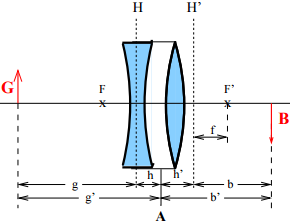
\includegraphics[height=6cm]{picture/Abbe}
	\caption{Schematische Darstellung für das Verfahren nach Abbe. \cite[5]{sample}}
	\label{fig:Abbe}
\end{figure}

Aus den Gleichungen
\begin{equation}
	g' = g + h = f \cdot \left(1 + \frac{1}{V} \right) + h
	\label{eqn:g'}
\end{equation}
und
\begin{equation}
	b' = b + h' = f \cdot \left(1 + V \right) + h'
	\label{eqn:b'}
\end{equation}
ergeben sich dann die Brennweite $f$ und die Lage der Hauptebenen. In den beiden obenstehenden Gleichungen ist $V$ der Abbildungsmaßstab und $h$ und $h'$ sind die Hilfsebenen.
